\begin{}
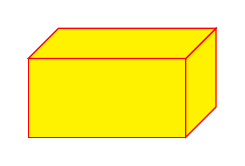
\begin{tikzpicture}
\pgfmathsetmacro{\cubex}{2}
\pgfmathsetmacro{\cubey}{1}
\pgfmathsetmacro{\cubez}{1}
\draw[red,fill=yellow] (0,0,0) -- ++(-\cubex,0,0) -- ++(0,-\cubey,0) -- ++(\cubex,0,0) -- cycle;
\draw[red,fill=yellow] (0,0,0) -- ++(0,0,-\cubez) -- ++(0,-\cubey,0) -- ++(0,0,\cubez) -- cycle;
\draw[red,fill=yellow] (0,0,0) -- ++(-\cubex,0,0) -- ++(0,0,-\cubez) -- ++(\cubex,0,0) -- cycle;
\end{tikzpicture}
